%% ---
%% GenGeo Section
%% ---
\chapter[GenGeo]{Jazzing things up: complicated particle geometries using \texttt{GenGeo}}

\section{A short introduction to \texttt{GenGeo}}
The \texttt{GenGeo} library is build around three basic concepts:
\begin{itemize}
\item geometrical volumes to fill with particles  
\item a "Packer" to place the particles into the volumes according to given criteria 
\item the "Neighbour Table" - a container to store the particles and to keep track of their relative positions and neighbour relations 
\end{itemize}

\subsection{Volumes}

\subsection{Packers}
While the library is designed to be flexible and to allow many different packing methods to be included the only packers implemented at the moment are all based to the insertion-based algorithm described in (REF). The advantages of this packing strategy are that it produces relatively dense particle arrangements where each interior particle is touched by at least 4 other particles in 3D (by 3 other particles in 2D) and that there are no frozen-in stresses between the particles. The disadvantage is that the user can not control the particle size distribution except for the minimum and maximum particle radius allowed.  

\subsection{Neighbour Tables}
- Verlet \\
- 2D/3D \\
- Circular Boundaries \\

\section{Particles in a box: a simple \texttt{GenGeo} example}
\label{sec:simple_box}

This section introduces the basic features of \texttt{GenGeo} using a very simple example: filling a box with particles. The resulting particle packing is similar to that produces inside the ESyS-particle simulation described in section \ref{sec:block_in_sim}. However, given that it is saved to a file it can be re-used for multiple simulations. The full code for the example is available in Appendix~\ref{geocode:box}. N.B. To make the meaning of the function arguments clear the "named argument" style of python function calls will be used in the sections explaining the \texttt{GenGeo} example. However, to improve general readability the compact form, i.e. without argument names, will be used for the full listings in the appendix. \par
Like most simple \texttt{GenGeo} scripts this example consists of 5 steps:
\begin{enumerate}
\item setting up a neighbour table
\item defining the volume to be filled - i.e. the box
\item setting up the packer
\item running the packer to fill the box and, if required, bond the particles together
\item write the particle data to an output file 
\end{enumerate}  
As usual, the thing to do in a python script is to import the necessary modules, therefore the script to pack particles into a box starts with 
\begin{verbatim}
from gengeo import *
\end{verbatim}
which of course assumes that the  \texttt{GenGeo} library \footnote{Despite the fact that it is spelled \texttt{GenGeo} throughout this tutorial, the actual module name is all lower case \texttt{gengeo}, i.e. on Unix systems the shared library name is gengeo.so } is in the python path. In order to make the code more readable we first define a couple of parameters which will be needed repeatedly throughout the script, namely the dimensions of the box we intent to fill and the minimum and maximum radius of the particles. For simplicity we place one corner of the box at (0.0,0.0,0.0) so we only need to specify the x-, y- and z- extent of the box to define it fully \footnote{The "Box" volumes, both in 2D and in 3D, only support boxes with edges parallel to the coordinate axes. Non-axis aligned boxes can be defined using a convex polyhedron volume.}. So the next section of the script looks like this:
\begin{verbatim}
# box dimensions
xdim=10
ydim=20
zdim=10

# particle size range
minRadius = 0.2
maxRadius = 1.0
\end{verbatim}
This will set the shape of the box to a square prism two times as long as wide. This shape is quite often used, for example in simulations of triaxial deformation tests. With the parameters given here the resulting model will be relatively small ($\approx 4000$ particles) and should build in about 10 - 20 seconds on current PC \footnote{Tested $\approx 16$ seconds on an Intel Core2 Q9300 (2.5GHz)}. For convenience we also define the two opposing corners of the box as vectors. N.B. In \texttt{GenGeo} the class for a 3D vector is called \texttt{Vector3}, \emph{not} \texttt{Vec3} as in ESyS-Particle! The reason for this difference is to avoid name conflicts when using both \texttt{GenGeo} and ESyS-Particle libraries in the same Python script. So the definition of the corner points is
\begin{verbatim}
# corner points
minPoint = Vector3(0.0,0.0,0.0)
maxPoint = Vector3(xdim,ydim,zdim)
\end{verbatim}
Now the corner points can be used to define both the volume to be filled and the neighbour table to contain the particles. The volume, which is of the class \texttt{BoxWithPlanes3D} takes exactly two parameters in its constructor, describing the locations of two opposite corners of the box. Therefore both parameters are of type \texttt{Vector3}. The class name \texttt{BoxWithPlanes3D}, in particular the "WithPlanes" part will become clearer in the next section \ref{sec:gengeo_box2}.
So to set up the box we use the previously defined corner points
\begin{verbatim}
# block volume
box = BoxWithPlanes3D(
    minPoint=minPoint,
    maxPoint=maxPoint
    )
\end{verbatim}
Next we need a neighbour table to store the particles. The constructor for the neighbour table takes 4 arguments: two corner points (\texttt{minPoint}, \texttt{maxPoint}) to describe the volume covered by the model, the grid spacing (\texttt{gridSize}) and the number of particle groups (\texttt{numGroups}). The volume covered by the neighbor table should ideally be the bounding box of the whole model, i.e. it needs to cover all particles but it should not be much larger in order to minimize the memory used. The grid spacing determines the search range used for the determining if two particles touch each other. To make sure all touching (or intersecting) pairs of particles can be found the grid spacing needs to be larger than twice the maximum particle radius. The number of particle groups will only be different from 1 for rather complicated geometry set-up scripts, so we set numGroups=1 here. So the construction of the neighbor table looks as follows:
\begin{verbatim}
# neighbour table 
mntable = MNTable3D(
    minPoint=minPoint,
    maxPoint=maxPoint,
    gridSize=2.5*maxRadius,
    numGroups=1
    )
\end{verbatim}
Next we need to set up the "packer" which places the particles inside the volume. As we want to pack single particles in 3D we chose a packer of type \texttt{InsertGenerator3D}. The most simple constructor for this type of packer takes 5 arguments. In addition to the minimum and maximum particle radius (\texttt{minRadius}, \texttt{maxRadius}) there are 3 parameters which control the performance of the packing algorithm. These are the number of consecutive failed particle insertion attempts allowed before the algorithm gives up and terminates(\texttt{insertFails}), the maximum number of iterations for the internal sphere fitting procedure (\texttt{maxIterations}) and the precision of the sphere fitting, i.e. the maximum tolerance up to which two particles are still considered touching (\texttt{tolerance}). The values we use here, \texttt{insertFails=1000}, \texttt{maxIterations=1000} and \texttt{tolerance=1e-6} usually work fine for small to medium models. For large models it can be necessary to increase the value of \texttt{insertFails} to obtain a good packing. The value of \texttt{tolerance} should be considered in relation to the particle radii. A sixth parameter \texttt{seed} can be used to force a re-seeding of the random number generator before the packing algorithm starts.  Setting \texttt{seed=True} guarantees a different packing with each run of the script, what happens otherwise is system-dependent. Taking this all into account the packer is constructed like this:
\begin{verbatim}
# packer
packer = InsertGenerator3D(
    minRadius=minRadius,
    maxRadius=maxRadius,
    insertFails=insertFails,
    maxIterations=maxIter,
    tolerance=tol
    )
\end{verbatim}
Now that the volume, the neighbour table and the packer, are defined the actual work can start. First the packer needs to fill the volume with particles. In the simplest case this requires two arguments to the \texttt{generatePacking} function of the packer: the volume to fill and the neighbour table in which to store the particles. Therefore the function call to fill the "box" volume with particles is
\begin{verbatim}
# pack particles into volume
packer.generatePacking(
    volume=box,
    ntable=mntable
    )
\end{verbatim} 
The last thing to do to complete the generation of the particle arrangement is to create the bonds between touching particle pairs. Because the neighbour table contains all informations necessary to determine which particles should be bonded, i.e. particle positions and radii, the bonding procedure is a member function of the neighbour table. The most simple form of the function call, which just bonds all neighbouring particles in on group, needs 3 arguments: the ID of the particle group which should be bonded \texttt{groupID}, the bonding tolerance \texttt{tolerance} and the tag given to the newly created bonds \texttt{bondID}. Because our neighbour table contains only one group of particles, we need to set \texttt{groupID=0}. The tolerance for bonding should normally be larger than the packing tolerance used in the packer, so we chose 1e-5 here. The bond tag can be set to any value, but given that we only have one set of bonds in this model we may as well use 0. So the call to create the bonds looks as follows:  
\begin{verbatim}
# create bonds between neighbouring particles:
mntable.generateBonds(
    groupID=0,
    tolerance=1.0e-5,
    bondID=0
    )
\end{verbatim}
And after this the model is fully built. The only thing left to do is to write the model data into a file so it can be used. For this purpose the neighbour table has a \texttt{write} function which can write the information stored in the neighbour table, i.e. particles and bonds, to a file in different ways which are controlled by the \texttt{outputStyle} argument. If \texttt{outputStyle=1} a "geo" file is written which can be used in ESyS-Particle scripts, if  \texttt{outputStyle=2} a VTK file \footnote{Specifically a VTK-XML unstructured grid file - see the documentation of VTK toolkit on www.vtk.org for more details on the file format.} is written for the use with visualisation software such as Paraview(tm). Of course the \texttt{write} function also needs the file name as first argument, so to write both a geo and a VTK file the calls should be:
\begin{verbatim}
# write a geometry file
mntable.write(
    fileName="box.geo", 
    outputStyle=1
    )
mntable.write(
    fileName="box.vtu",
    outputStyle=2
    )
\end{verbatim}   
which concludes the \texttt{GenGeo} script to generate a box filled with bonded particles. The script can now be executed as usual, i.e. \texttt{python\ simple\_box.py}. During execution there will be some debug output, in particular for every 100 particles inserted \texttt{GenGeo} will output a line stating how many particles have been inserted so far \footnote{This number does not include the particles generated during the "seeding" stage of the algorithm} and how many attempts it took on average to insert one of the last 100 particles. When the execution of the script finishes it should have produces two files, "box.geo" and "box.vtu". When visualized with Paraview the result should look similar to that shown in Figure \ref{fig:simple_box}.  
%% --- Fig simple_box
\begin{figure}
\begin{center}
\resizebox{2.5in}{!}{
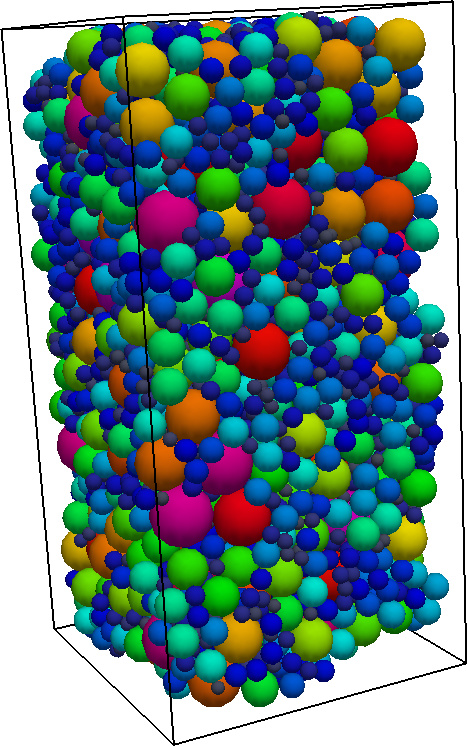
\includegraphics{gengeo_box.jpg}}
\end{center}
\caption{An image (generated with Paraview) of the box filled with particles generated by the script \texttt{simple\_box.py} described in section \ref{sec:simple_box} } \label{fig:simple_box}
\end{figure}
%% -----
One issue which is noticeable with this model is that the surfaces, and particularly the edges, are rough, rather than smooth. How to overcome this is described in the next section.

\section{Particles in a box Mk II: making the the boundaries smooth(er)}
\label{sec:gengeo_box2}
The reason why the walls of the box generated in the previous section are not as smooth as expected is that the \texttt{InsertGenerator} uses the box volume only determine if a particle is inside the volume or not, it does not fit particles to the faces of the box. This can be changed by adding some \texttt{Plane} objects to the box volume. To do this, it is necessary to define the planes first. Each \texttt{Plane} object is defined by a point on the plane and the normal direction of the plane. To add a  \texttt{Plane} object for each face of the box a total of 6 planes are needed, three passing through the point (0,0,0), which is called \texttt{maxPoint} in the script described in the previous section, with normals pointing in the positive x-, y- and z-direction and three passing through the opposite corner of the box, which was called \texttt{maxPoint} in the script. So the definition of a plane parallel to the xy-plane, i.e. with a normal pointing in the z-direction, and going through the point "minPoint" is
\begin{verbatim}
bottomPlane=Plane(
    origin=minPoint,
    normal=Vector3(0.0,0.0,1.0)
)
\end{verbatim} 
The other 5 planes can be defined in the same way or, more compact, by the following lines:
\begin{verbatim}
leftPlane=Plane(minPoint,Vector3(1.0,0.0,0.0))
frontPlane=Plane(minPoint,Vector3(0.0,0.0,1.0))
topPlane=Plane(maxPoint,Vector3(0.0,-1.0,0.0))
rightPlane=Plane(maxPoint,Vector3(-1.0,0.0,0.0))
backPlane=Plane(maxPoint,Vector3(0.0,0.0,-1.0))
\end{verbatim}
To enable the packer to fit the particles to the planes when filling the box volume the \texttt{Plane} objects need to be added to the \texttt{BoxWithPlanes3D} object by using its \texttt{addPlane} member function. This function takes a \texttt{Plane} object as its only argument. To add the bottomPlane defined above to the box volume the call is 
\begin{verbatim}
box.addPlane(
    Plane=bottomPlane
)
\end{verbatim}
and for the other five planes, in the compact form,
\begin{verbatim}
box.addPlane(leftPlane)
box.addPlane(frontPlane)
box.addPlane(topPlane)
box.addPlane(rightPlane)
box.addPlane(backPlane)
\end{verbatim}
If these lines are added \ref{sec:simple_box} somewhere between the definition of the box volume and the call to generate the particle packing in the simple script filling a box which was developed in the previous section we have the complete script to generate a box full of particles where the sides are as smooth as possible for the given particle size range. The full code for the example is available in Appendix~\ref{geocode:smooth_box}. The resulting model can be seen in Figure \ref{fig:smooth_box} A). If the surfaces are still too rough for a particular application the smoothness can be improved by extending the range of particle sizes towards smaller radii. This can easily be achieved in the script described here by changing the variable \texttt{minRadius} to an appropriate value. The result of setting  \texttt{minRadius=0.05} is shown in Figure \ref{fig:smooth_box} B). \par	

%% --- Fig smooth_box
\begin{figure}
\begin{center}
\resizebox{120mm}{!}{
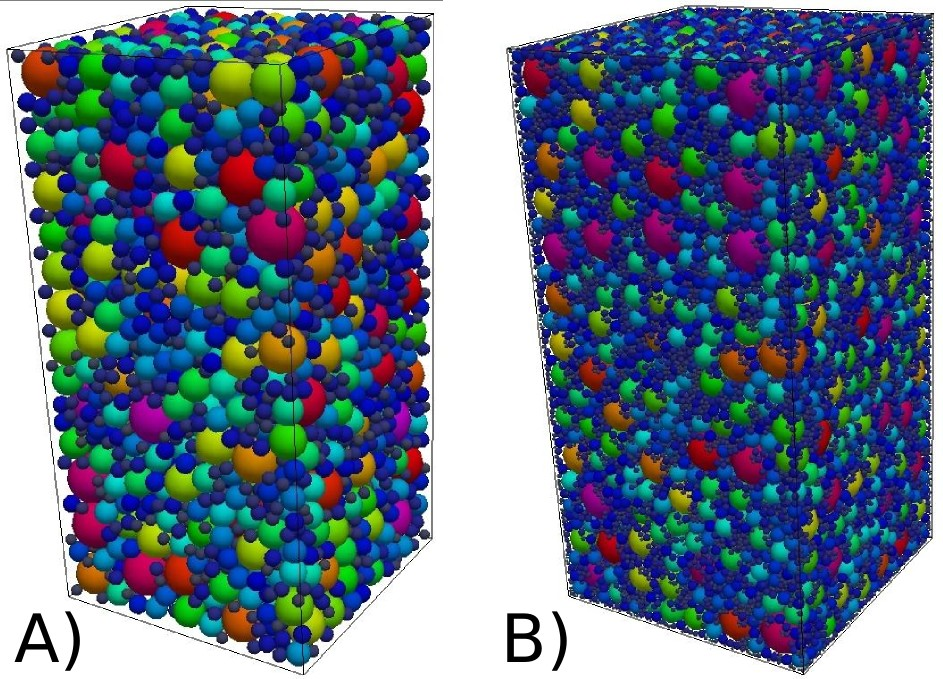
\includegraphics{smooth_box.jpg}}
\end{center}
\caption{Images (generated with Paraview) of a box with particles fitted to the box faces generated by the script \texttt{smooth\_box.py} described in section \ref{sec:gengeo_box2}. The model in A) uses particle radii between 0.2 and 1.0, the model in B) uses particle radii between 0.05 and 1.0.} \label{fig:smooth_box}
\end{figure}
%% -----

\subsection{Smoothness, particle sizes and particle numbers}

However, while smooth surfaces and dense particle arrangements can be realized with packings using wide size distribution of particles, i.e. a large ratio $r_{max} : r_{min}$ it should also be noted that this leads to a significant increase in the number of particles for the same model size. A very rough estimate would be that for a given maximum particle size the total number of particles in a volume goes up approximately as $n_p \approx 1 / {r_{min}}^2 $ \footnote{The exact relationship between model volume, particle size range and particle number is more complicated, particularly for relatively narrow particle size ranges. However, the $ 1 / {r_{min}}^2 $ relationship is a usable rule of thumb. N.B. This applies for \textbf{fixed} $\mathbf{r_{max}}$  - for fixed $ r_{max} / r_{min} $  the relation is obviously  $n_p \approx 1 / r^3 $ } where $n_p$ is the total number of particles. For the models shown in Figure \ref{fig:smooth_box} the total number of particles went up from about 5300 to 72000, representing an increase by a factor of 13.6 where the rule mentioned above would predict a factor of 16 for the reduction of the minimum particle radius from 0.2 to 0.05. \par
A second issue which needs to be taken care of when using large particle size ranges is that in the definition of the \texttt{InsertGenerator3D} the maximum number of attempts to insert a particle should be increased. The rationale behind this is that the packer now needs to find smaller "holes" in which to insert particles so it needs to try more often. The model shown in Figure \ref{fig:smooth_box} B) was generated using \texttt{insertFails = 10000}. There is unfortunately no hard rule how many attempts to insert a particle should be used for a specific combination of volume and particle size range. A possible way to find a suitable number of insertion attempts for a specific problem is to re-run the packing script a couple of times with different values \texttt{insertFails} and observe how the density of the packing changes. A good way to measure the packing density is to calculate the porosity of the model. This can be done by calculating the combined volume of all particles using the \texttt{getSumVolume} member function of the neighbour table and subtracting this from the total model volume. For the box this can be calculated easily as the product of the x-, y- and z-dimension like
\begin{verbatim}
volume = xdim*ydim*zdim
porosity = (volume - mntable.getSumVolume(groupID=0))/volume
\end{verbatim}
where the \texttt{groupID=0} argument to the \texttt{getSumVolume} call determined to which group of particles in the neighbour table it is applied. While a comprehensive discussion of the influence of the packing parameters on the resulting particle arrangement is beyond the scope of this manual, a reasonable rule to make sure a dense packing is obtained for a given problem is to use such a value of \texttt{insertFails} that the change of model porosity resulting from a doubling of \texttt{insertFails} is of a similar order as the porosity variations between different realizations of the model.
  
\section{Getting serious: groups, particle tags and bond tags}

\section{Grouping particles: a box of clusters}
\label{sec:gengeo_clusterbox}

For some types of simulations it can be useful if the particles in the model are grouped into grains or "clusters" where the intra-cluster bonds do have different properties than the bonds between the clusters \footnote{Strictly speaking, the bonds between particles belonging to different clusters.}. The approach for generating such a particle arrangement described in this section has for example been used by Abe and Mair, GRL 2009 \cite{Abe_Mair_GRL_2009}. This example also demonstrates how to use a number of particle groups in the neighbour table is greater than 1. To simplify the script here only a single box is filled with particle clusters. The full code for the example is available in Appendix~\ref{geocode:cluster_box}. \par
The key ideas of the particle clustering approach described here are:
\begin{enumerate}
\item The clustering happens after the particle packing.\footnote{Approaches defining the clusters before packing the particles are also possible but much more complicated and not within the scope of this manual.}
\item There are a number of "seeds" distributed within the volume
\item Each particle is tagged depending on which of the seeds is closest to it
\item When generating the bonds, bonds between particles with different tags get a different tag than bonds between particles with the same tag \footnote{Careful not to mix up particle tags and bond tags here!}
\end{enumerate} 
Point 1. above means that the box filling script from section \ref{sec:gengeo_box2} can be used as a starting point, with just some small changes. In particular the number of particle groups in the neighbour table needs to be 2 instead of one, i.e. the construction of the neighbour table becomes
\begin{verbatim}
mntable = MNTable3D(
    minPoint=minPoint,
    maxPoint=maxPoint,
    gridSize=2.5*maxRadius,
    numGroups=2
    )
\end{verbatim}
The next step is to generate a number of seed points distributed in the volume. For simplicity we just arrange them in a regular grid here. In a production model a more complicated arrangement of the seed points is usually needed, for example adding some random displacement to the regular grid. First we specify the parameters of the regular grid, in this case for a 3x6x3 arrangement of the clusters, i.e. we specify the number of clusters in each direction and calculate the dimensions of the clusters from the size of the box and the number of clusters per dimension. It would also be possible to do this the other way around, but doing it this way guarantees that the clusters fit into the box, i.e. we do not get smaller clusters at the edges of the box. If that would be an issue will depend on the specific application the model is used for.  
\begin{verbatim}
ncluster_x=3
ncluster_y=6
ncluster_z=3
dx=xdim/float(ncluster_x)
dy=ydim/float(ncluster_y)
dz=zdim/float(ncluster_z)
\end{verbatim}
With these parameters a set of nested loops can be used to calculate the positions of the seeds 
\begin{verbatim}
for i in range(ncluster_x):
    for j in range(ncluster_y):
        for k in range(ncluster_z):
            x=(float(i)+0.5)*dx
            y=(float(j)+0.5)*dy
            z=(float(k)+0.5)*dz
            seed_pos=Vector3(x,y,z)
\end{verbatim} 
To tag each particle according to the seed closest to it the neighbour table member function 
\texttt{tagParticlesToClosest} can be used. However, this function operates on two sets of particles in the neighbour table, assigning tag of the closest particle in on group to the particles in the other group. This means that the "seeds" actually need to be particles in the neighbour table. However, because the seed particles are just dummy particles and must not interact with the "real" particles they can not be simply inserted in the neighbour table. This is where the concept of multiple particle groups becomes useful: if the seed particles are inserted in a different particle group than the real particles they are still part of the same neighbour table so member functions can operate on them, but they otherwise do not interfere with each other. So the way to insert the seeds into the neighbour table is to construct a particle, i.e. a \texttt{Sphere} object for each seed, give it an appropriate tag and insert it into group 1 \footnote{The other "real" particles are in group 0 - the \texttt{generatePacking} call places them there by default.}. The constructor of a \texttt{Sphere} object takes two parameters, the center of the sphere, which is of type \texttt{Vector3}, and the radius of the sphere, which is a \texttt{float}. Here a radius of 0.0 is used for the seed particles.
\begin{verbatim}      
            # construct & insert seed "pseudo-particle"
            cseed=Sphere(seed_pos,0.0)
            tag=i*ncluster_y*ncluster_z+j*ncluster_z+k
            cseed.setTag(tag)
            mntable.insert(cseed,1)
\end{verbatim} 
These instructions are still part of the loop above, so they have to be indented accordingly (see full code at Appendix~\ref{geocode:cluster_box}). The tags of the seed particles are generated from the loop variables making sure there is no duplication.\par
This completes the preparation for the generation of the clusters. The only things left to do are to tag the particles according to the seeds and to generate the bonds. The tagging is done using the \texttt{tagParticlesToClosest} function mentioned above. This function takes two parameters: first the number of the group in which the particles are tagged, i.e. the real particles, and second the group from which the tags are taken, i.e. the seed particles. The bonds are generated using the \texttt{generateClusterBonds} member function of the neighbor table. Similar to the simple \texttt{generateBonds} function it takes a \texttt{GroupID} and a \texttt{tolerance} argument, but instead of a single bond tag argument it takes two of those, \texttt{bondTag1} for bonds between particles with the same tag, i.e. the intra-cluster bonds, and \texttt{bondTag2} for bonds between particles with different tags. If the tag for intra-cluster bonds is set to 1 and the tag for the bonds between clusters is 2, the code is
\begin{verbatim}
# tag particle according to nearest seed
mntable.tagParticlesToClosest(
    groupID1=0,
    groupID2=1
)

# generate bonds
mntable.generateClusterBonds(
    GroupID=0,
    tolerance=1.0e-5,
    bondTag1=1,
    bondsTag2=2
)
\end{verbatim}
Because the seed particles are not part of the actual model geometry they should be removed before writing the geometry to a file by calling 
\begin{verbatim}
mntable.removeParticlesInGroup(
    GroupID=1
)
\end{verbatim} 
where the \texttt{GroupID} parameter is the number of the group for which all particles are removed \footnote{This requires at least rev. 120 of GenGeo. For older versions this has to be done less elegantly by calling \texttt{mntable.tagParticlesInGroup(1,1)} to set the tag of all particles in group 1 to 1 and  \texttt{mntable.removeTaggedParticles(1,1,-1)} to remove them.\footnotemark}. \footnotetext{N.B. There is a bug in \texttt{removeTaggedParticles} in GenGeo versions prior to rev. 120 which prevents the use of a tag, mask combination fitting all tags, i.e. 0,0, to achieve the same result.} This completes the script to fill a box with particles and to bond them together in clusters. The resulting model is shown in Figure \ref{fig:cluster_box}. 

%% --- Fig cluster_box
\begin{figure}
\begin{center}
\resizebox{120mm}{!}{
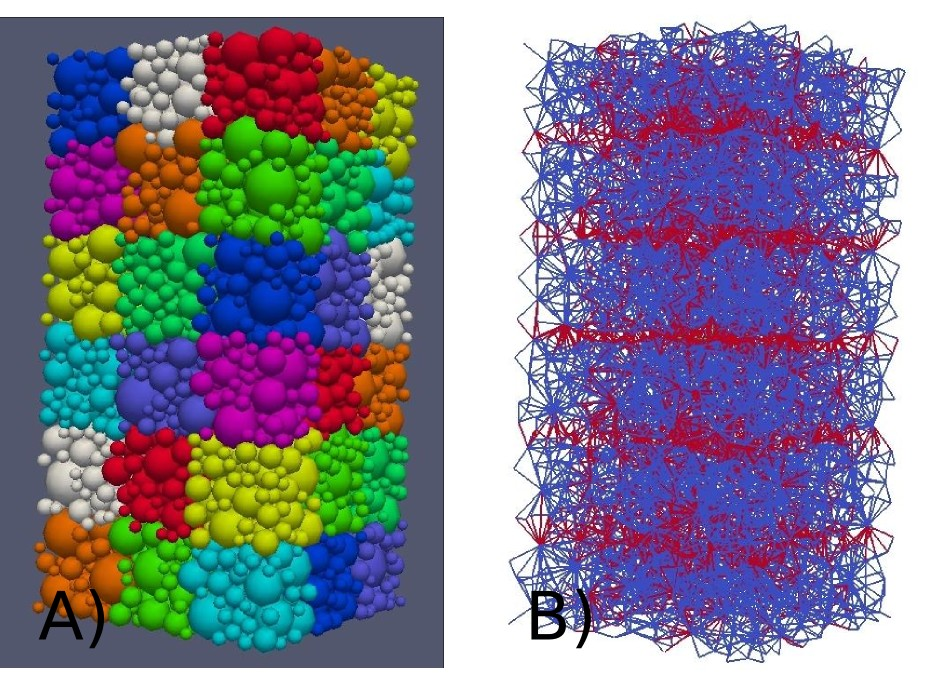
\includegraphics{cluster_box.jpg}}
\end{center}
\caption{Images (generated with Paraview) of a box with clustered particles generated by the script \texttt{cluster\_box.py} described in section \ref{sec:gengeo_clusterbox}. Panel A) shows the particles colored by particle tag. To enhance the visual contrast between neighboring clusters colors are set using particle tag modulo 10.  Panel B) shows the bonds in this model. Intra-cluster bonds (bond tag 0) are shown in blue and tags between clusters (bond tag 1) in red.} \label{fig:cluster_box}
\end{figure}
%% -----

\section{Lateral thinking: hierarchical packing for complex models}

\section{If nothing else helps - the \texttt{MeshVolume}}
\label{sec:mesh_volume}

For complicated geometries which can not be reasonably expressed as combination of simple volumes there is a way to fill any volume bounded by a closed, triangulated surface with particles. However, it should be noted that this can be computationally rather expensive, in particular that the computation time goes up roughly linear with the number of triangles forming the surface. On the other hand, it is usually faster than constructing the same volume from a set of convex polyhedra. Also, it should be noted that there is currently no facility to import any given mesh format into \texttt{GenGeo}. 

\section{What else is there?}
This section provides short descriptions of the remaining features of the \texttt{GenGeo} library. Features marked \textit{EXPERIMENTAL} may not be completely implemented and / or tested yet and therefore have bugs and limitations.   
 
\subsection{Volumes}
\subsubsection*{BoxWithJointSet}
\subsubsection*{ConvexPolyhedron}
\subsubsection*{SphereVol}
\subsubsection*{ClippedSphereVol}
\subsubsection*{CylinderVol}
\subsubsection*{CylinderWithJointSet}
\subsubsection*{DogBone}
\subsubsection*{EllipsoidVol \textit{EXPERIMENTAL}}
\subsubsection*{Constructive Solid Geometry (CSG) based volumes \textit{EXPERIMENTAL}}
\subsubsection{Objects}
\subsubsection{Tagging and Bonding}
\section*{What's Next?}